

\documentclass[conference]{IEEEtran}
\hyphenation{op-tical net-works semi-conduc-tor}
\usepackage{booktabs,caption,fixltx2e}
\usepackage[flushleft]{threeparttable}
\usepackage{algorithm}
\usepackage{algpseudocode}
\usepackage{pifont}
\usepackage{setspace}
\usepackage{adjustbox}
\usepackage{graphicx}
\usepackage{svg}
\usepackage{amsmath}
\usepackage{multirow}
\usepackage{subfig}
\usepackage{footnote}
\usepackage{caption}
\usepackage{adjustbox}
%\usepackage[margin=1cm]{caption}

\usepackage{color}

\newcommand{\todo}[1]{\textcolor{red}{@TODO: #1}}
\begin{document}

\title{Amazon Wishlists}


\maketitle

\begin{abstract}
Online user behavior has been largely studied in various fields due to the prosperity of Internet. In this paper, we investigate Amazon Wishlists, where users keep their desired products for easier access or providing guidelines to gift givers. We collected Wishlists and items of over 30,000 users, in the mean time showing interesting results on user online shopping behavior. Specifically, we show behavior difference in gender and geo-location. Besides, we also study shopping patterns in normal days and holidays. Surprisingly we found that user may not always like to shop during holidays. Finally, we demonstrate that information in Wishlists has potential to leak user personal information. We use state-of-art machine learning techniques (SVM) to train and test the data. Our result indicates that based solely on the items in users' Wishlists, their gender, education, and hobbies can be inferred with a considerable success rate. 
\end{abstract}
\section{Introduction}
Entering the era of big data, Internet has been instantly extended to be data-rich. User data can be exploited to generate large benefit in many fields. Electronic commerce is one of the most data-driven market. There have been many works studying how users behave or user reactions in E-commercials \cite{tsai2011effect, ghose2011estimating, ivanova2013does}. Studying user behaviors in e-commercials help understanding the market and thus generate better economic outcomes. For example, user data can be monetized by feeding targeted advertising or performing price discrimination~\cite{mikians2012detecting}. Although there are various kinds of user data on Amazon, user shopping history and preference is one of the most sensitive and valuable type of data. However, shopping history is considered private information that most users do not wish to publicize. To cope with user expectations, most e-commerce companies keep user shopping history private. Therefore, a major challenge of studying shopping preference is to collect data from users. Nonetheless, users may not always hide their purchase intentions. Wishlist, a list-type data in Amazon, is made publicly available by default. Users add items in their wishlists to record desired products for their own reference or for gift givers. As users use wishlists to record desired products, wishlists largely reflect the shopping preference of users -- If a user adds a item in his/her wishlist, the user is likely to buy the item or make other people buy the item. Besides, wishlists are also indicators of shopping history since the items will not be removed after the item is bought unless manually deleted.

As the world's leading e-commerce company, Amazon is a particularly important source for understanding user shopping behaviors. In this paper, we analyze wishlists in Amazon to study user shopping patterns as well as the privacy implication of wishlists. By doing so we shed light on general user preference on e-commerce and help companies to refine both their marketing strategies and privacy policy.

We first collected complete profile and wishlists information of over 30,000 users and approximately 2 million items in Amazon by web scraping. Based on the data, we conduct measurement study on user behaviors. Our study concentrates on user shopping preference, which are organized in 3 dimensions — 1)Product Categories 2)Product prices 3) Timing. Specifically, we compare the user preference in different gender and regions. We also investigate shopping pattern in different time through a year. Surprisingly we found that there is little shopping increase in holidays or weekends and even some holidays are shopping repelling. We believe our findings provide insight that is able to help sellers to revise their marketing strategies, as well as to help advertisers to make more accurate targeted advertising. 

Beside user behavior analysis, we study user privacy information exposure in Amazon. Network users are prone to expose their private information in public websites inadvertently~\cite{frankowski2006you, friedland2010cybercasing}, making themselves face the threat of information leakage. Privacy protection is very important for websites not only because it involves legal issues but also that it correlates to user purchasing intentions~\cite{brown2004investigating, tsai2011effect}. To study to what extent does the information in wishlists threat user privacy, we investigate both the items in wishlists and the user input list-descriptions to identify user personal information. We first illustrate user personal information exposure by analyzing their list-descriptions, showing that users are mentioning sensitive personal information such as profession, education background, relatives' information, etc in their list-descriptions. 

Furthermore, public information may be exploited to infer user personal information. Such information leakage has been proved in many works~\cite{narayanan2009anonymizing, wondracek2010practical, chaabane2012you, hecht2011tweets, goga2013exploiting}. In our study, we also try to identify user personal information leakage through analyzing publicly available data. Specifically, we use Support Vector Machine (SVM) to predict user gender based solely on items in their wishlists. The result indicates that user gender information can be identified with fairly high accuracy.  

\section{Data and Methodology}
As the largest electronic retailer in the U.S, Amazon was reported to have 270 active customer accounts in 2014 (http://www.statista.com/statistics/237810/number-of-active-amazon-customer-accounts-worldwide/). With such large user base, user behavior in Amazon significantly imply the market pattern and preference, which is critical for electronic commercials and advertisement ecosystem. However, such online user behavior has not been systematically studied before. In this paper we unveil customer shopping pattern in Amazon through analyzing Wishlists of a large amount of users.

Every registered user in Amazon has a public profile that contains various objects such as profile photo, rated items, reviews, and Wishlists, etc. Wishlist is a list-type object that contains the desired products added by the user. A user may have multiple Wishlists to accommodate different types of products. Wishlists can be useful in many ways. For examples, a user may use Wishlists to record the products he/she wishes to buy in the future. Or the user may use the Wishlist to show guidelines for gift givers. Beside items, each wishlist maintains a separate recipient profile, including name, birthday, and shipping address. When a new Wishlist for the user is created, birthday and address are defaulted to be empty, and recipient name is pre-set as the user's profile name. To preserve user privacy, birthday has only month and day in a Wishlist, thus the age of the recipient is unknown. Similarly, address information shows only the state and city. Note that although every user has a public profile, not all objects in this profile are public. Wishlists are configurable yet public in default. We focus on the analysis of user Wishlists. Therefore, other objects that are beyond the scope of this paper such as reviews, activities are deliberately omitted.

Figure~\ref{data_struct} shows the data hierarchy in our measurement. We illustrate only the layers under the Wishlist. As we can see from the figure, other than items, each list has its own recipient name, birthday, and address. Beside these formated information, each Wishlist can have a list-description. List-description is plain text keyed in by the users, which is which is usually used to briefly introduce the wishlists and the users. Examples are \emph{``I LOVE music! Buy me a CD!"} or \emph{``Son of Sue and Kevin, brother of Roger, husband of Kathy. I moved from Milton Keynes, England to Smithfield, North Carolina, USA on 8/8/2000 and recently moved from there to the Raleigh/Garner border in the same state"}. The first example list-description shows the hobby of a user and the second example exposes much more personal information such as parents' names, marriage status, wife name, moving history, etc. 

\begin{figure}[h!].
\centering
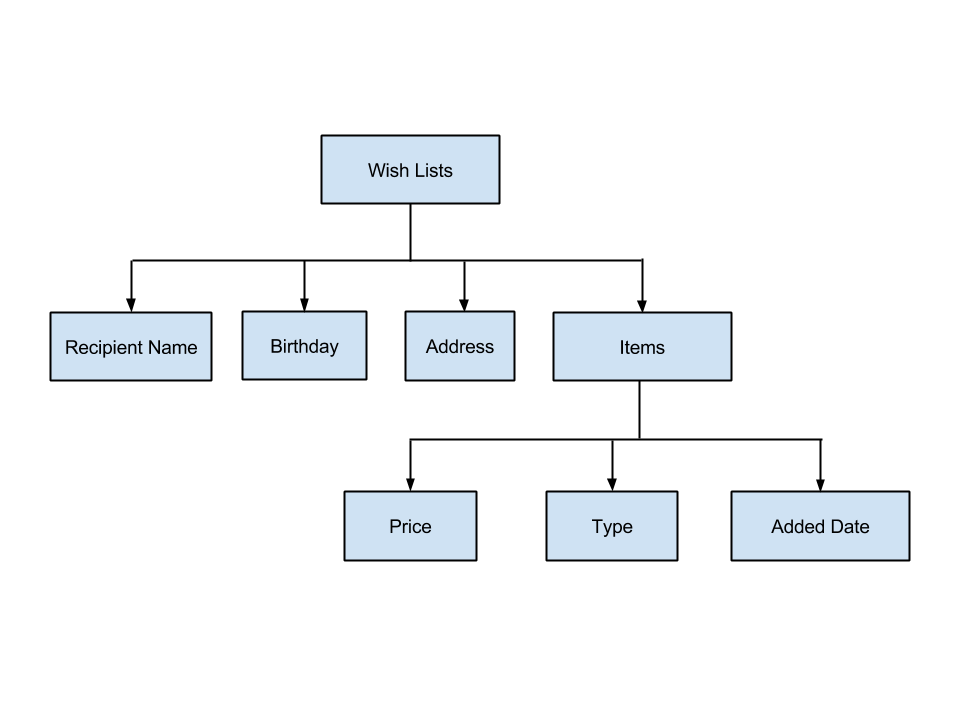
\includegraphics[width=.45\textwidth]{data_struct.png}
\caption{data hierarchy}.
\label{data_struct}
\end{figure}

As the Wishlist stores the user desired products, it directly reflect the user online shopping pattern in Amazon. Particularly we are interested in the products users prefer to buy, the time when shopping peak or pit happens, and the price users are willing to pay. Therefore we need to collect adequate number of data from Amazon for analysis. 

\subsection{Data Collection Methodology}
One way to collect data from Amazon is to use its Product Advertising API[]. However, the API does not provide wishlist or product type accesses, which are essential in our study. Besides, there is a 1 request/second limit on non-profiting API users (The actual rate is $1 + round({S\over \$4600})$[], in which $S$ denotes the sales in the user's website in last 30 days). Using few API accounts does not boost the speed while signing up for more accounts require much more effort. Therefore we opt for crawling Amazon by web scraping. Although web scraping may not be reliable, it provides all information that are needed. We implement the crawler using python package BeautifulSoup [] to extract specific data in certain HTML tags. 

Generally the data collection process consists of 3 steps. In each step we store certain data and collect input data for the next step. 

First we aim to collect substantial amount of user profiles to expand our crawling targets. From the user profile, we are able to extract the user name, birthday, address, Wishlist names, list URLs, and Wishlist list-descriptions. To this end, we leverage Amazon wishlist search engine~\cite{searcheng} to search common names. The wishlist search engine will return at most 2016 users and that are associated with a name. \footnote {The search engine usually states that hundreds of thousand users are found, but only the first 2016 users are viewable.} We have mentioned that each Wishlist under a user profile may have different personal information such as name, address, etc. The search engine returns the user name, birthday, address, and list-description as the ones in the latest updated Wishlist. Figure~\ref{searcheng} shows the result of a typical search, in which we searched user named ``Paul".


\begin{figure*}[!htb]
\minipage{0.32\textwidth}
  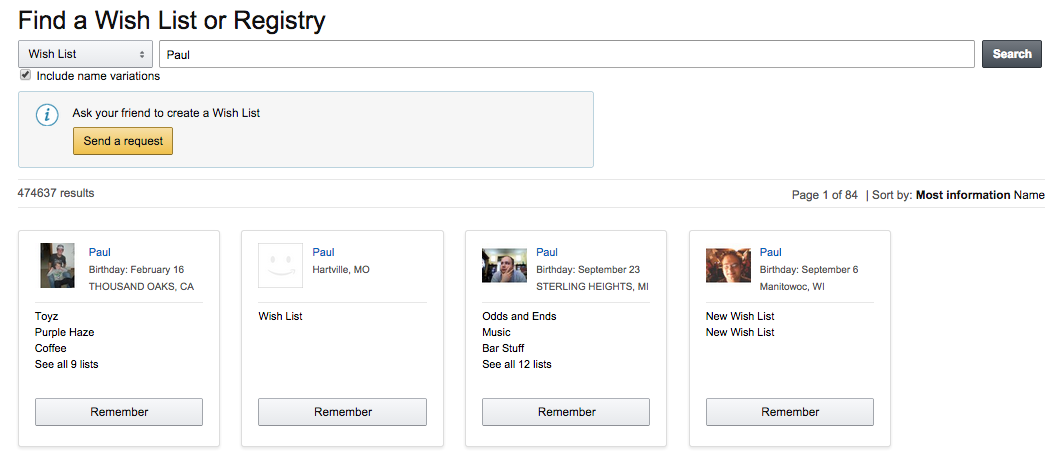
\includegraphics[width=\linewidth]{searcheng.png}
  \caption{Wishlist Search Engine}\label{searcheng}
\endminipage\hfill
\minipage{0.32\textwidth}
  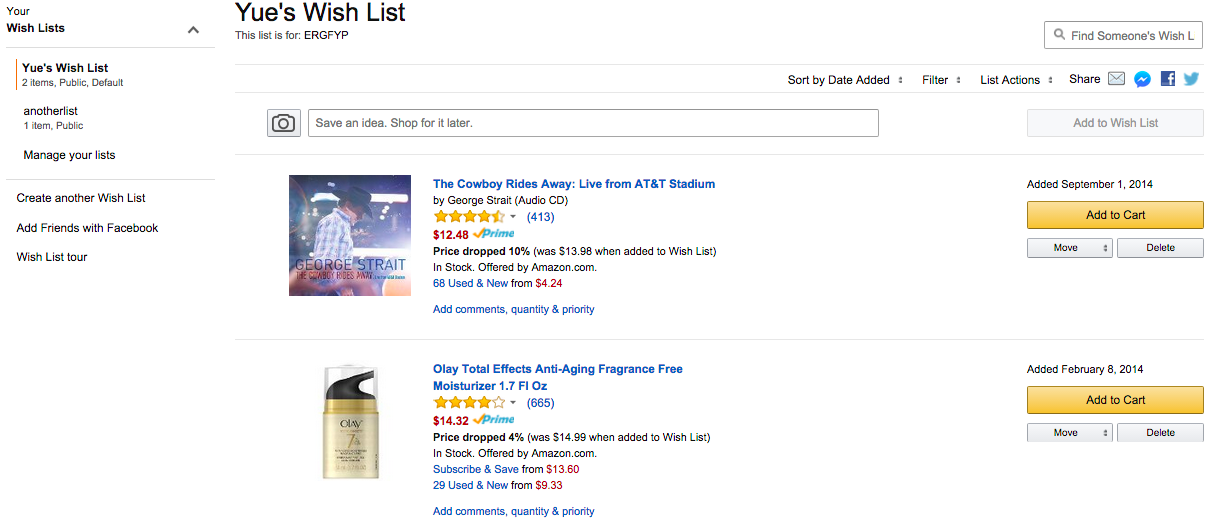
\includegraphics[width=\linewidth]{listitem.png}
  \caption{Wishlist}\label{listitem}
\endminipage\hfill
\minipage{0.32\textwidth}%
  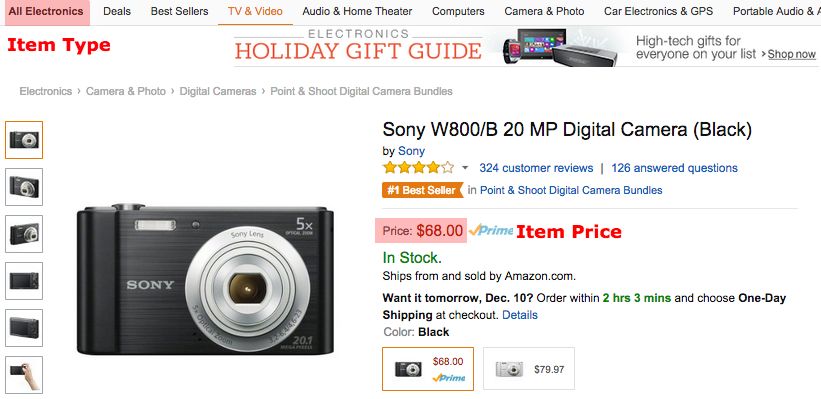
\includegraphics[width=\linewidth]{item.png}
  \caption{Item}\label{item}
\endminipage
\end{figure*}

Then we further investigate the items in the Wishlist. We directly visit the Wishlist URLs extracted in last step. In the page of Wishlist as shown in Figure~\ref{listitem}, the items are listed with links to their own pages. We cannot know the price and type of the item until we visit these pages. Therefore to this point we are only able to collect item name, item page URL and the date the items were added. 

Finally We retrieve detailed information for each item. We visit all the item URLs and download the product pages. One example of the product web pages is shown in Figure~\ref{itempage}. In a page like this, the item type and the item price (In red box) can be easily extracted. However, there may not always be only one price for an item. For example, for the same item, there can be prices from different retailers. There are also differences between new ones and used ones. We record only the price that the wishlist owner chose (Wishlists remember which version of the items are selected in most cases). In cases which the user does not choose a price, we record the lowest prices that a user needs to pay to get an item. In these rare case we believe it is reasonable to choose the lowest price because it is natural to assume that people prefer to pay less to purchase an item. Note that we cannot always find the price for an item. There are multiple reasons -- (1) The item is removed from Amazon so there is no web page for it. However, it still stays in user Wishlists. (2) The item is no longer in stock, the price shown will be ``Currently unavailable" (3) Web failures and anti-crawler mechanisms.

\subsection{Data Overview}
We searched the top 600 common names (300 males \cite{mnames} and 300 females \cite{fnames} to harvest user profiles. Eventually we collected 1,233,095 unique users.Their profile information and wishlist links are stored in our database. However, collecting Wishlists of all the users is very time-consuming (Consider that one Amazon product Page usually has over 10 thousand lines of code, which is around 300KB data). Therefore we collect only part of the user profile pool that is large enough to conduct sound measurement. As we are also interested in personal information of a user, we collect the wishlists and items of users who potentially have input personal information -- users with list-description. To this end, we collected 30,057 complete user, together with all the items and wishlists. In total we collected 76,923 wishlists and 5,710,674 items, among which 2,248,142 are unique. The size of the data is approximately 1.6GB. "MENTION MALE AND FEMALE NUMBER". 


\subsection{Personal Information}
Although we did not collect wishlists for all the recorded users. We can still use their wishlist profile to study personal information exposure in Amazon especially when we are particularly interested in potential user information leakage. Table~\ref{tb:stat} illustrates information exposure in user list profiles. We found that a considerable number of users put their birthday and location information in their list profiles. Furthermore, most of the people who have a list-description have exposed their birthday and address information. Our findings agree with \cite{frankowski2006you}, which states that users tend to expose their personal information in open websites. 

\begin{table}[!htbp]
\centering
\caption{Personal Information in User Profile}
\label{tb:stat}
\begin{adjustbox}{max width=.5\textwidth}
\begin{tabular}{lll}
Personal Info & User Number & Percentage \\
Birthday & 280,328 & 29.0\% \\
Location & 221,298 & 22.9\% \\
Birthday \& Location & 150,004 & 15.5\% \\
List-description & 104,846 & 10.8\% \\
List-description \& Birthday & 94,284 & 9.7\% \\
List-description \& Location & 59,731 & 6.2\% 
\end{tabular}
\end{adjustbox}
\end{table}


\section{Data Analysis}

Now we aim to dissect our dataset to reveal how users use their wishlists. Particularly we are interested in the products user prefer to buy, as well as the time that is appealing to shoppers. We compare user preferences in 3 different regions to show market trend. Besides, we also quantify the increase in different time of a year. Specifically we show different shopping behaviors in various holidays.

\subsection{Basic Statistics}
First we conduct fundamental measurements on the dataset to help build basic understanding on how wishlists are used and to what extend the users expose their personal information in Amazon. 

For all 967,603 users collected in the first step of data collection, we record totally 2,121,173 wishlists and 5,700,000 items (in which 2,248,142 items are unique). We show distribution metrics in Table~\ref{tb:stat2}. As we can see from the table, every user has 2.56 wishlists in average with standard deviation of 4.97. The average number and standard deviation of items in a wishlist is 74.2 and 187.3 accordingly. And the average and standard deviation of product price is \$35.06 and 172.0. Note that although we list the maximum number of wishlists a user has (Similarly, items in wishlists and item price) in our dataset, we did not probe the limit set by Amazon. All three distributions have very high skewness~($\gamma_1$) and kurtosis~($\kappa$), which means the distributions are very skewed and heavily tailed. For clearer presentation, we show the distribution of wishlist in Figure~\ref{avglist}, distribution of items in Figure~\ref{avgitem}, and distribution of price in Figure~\ref{avgprice} using log-scaled y axis.

\begin{table}[!htbp]
\centering
\caption{Distributions}
\label{tb:stat2}
\begin{adjustbox}{max width=.5\textwidth}
\begin{tabular}{llllll}
Distribution & Mean & Max & SD & $\gamma_1$ & $\kappa$ \\ \hline
Wishlist in Profile & 2.56 & 326 & 4.97 & 19.7 & 854.15 \\
Items in Wishlist & 74.2 & 7,350 & 187.3 & 8.25 & 111.11 \\
Item Price & 35.06 & 105,065 & 172.0 & 299.4 & 144,743.2 \\
\end{tabular}
\end{adjustbox}
\end{table}

\begin{figure*}[!htb]
\minipage{0.32\textwidth}
  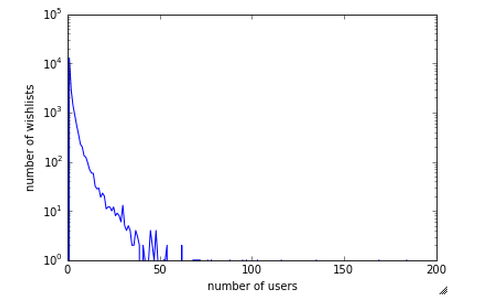
\includegraphics[width=\linewidth]{avglist.png}
  \caption{Number of lists the users have}\label{avglist}
\endminipage\hfill
\minipage{0.32\textwidth}
  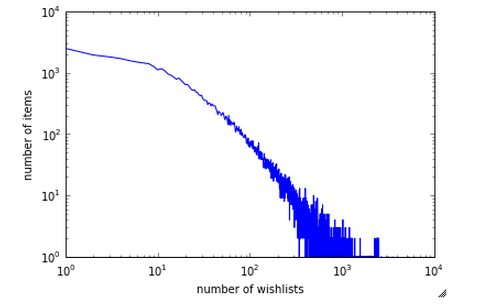
\includegraphics[width=\linewidth]{avgitem.png}
  \caption{Number of items the lists have}\label{avgitem}
\endminipage\hfill
\minipage{0.32\textwidth}%
  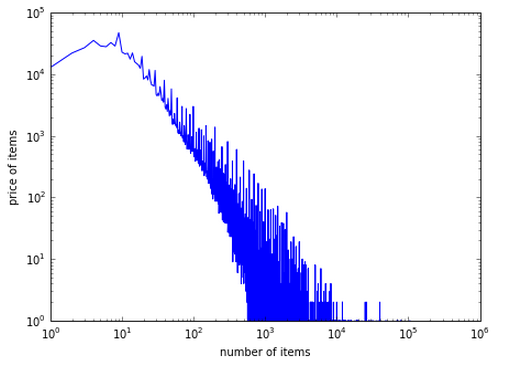
\includegraphics[width=\linewidth]{avgprice.png}
  \caption{Item Price}\label{avgprice}
\endminipage
\end{figure*}


\subsection{User preference}
A core question on user preference is what the users would like to buy and how much they are willing to pay for certain products. To categorize the products, we directly use item type that are in the product pages (See Fig~\ref{item}. From all product pages that are visited we found 50 types in total. Note that Amazon was reported to do price discrimination on E-books~\cite{mikians2012detecting}, which indicates a same E-book may be priced differently in various locations. However, these locations are in scope of countries. In our study, we focus on the U.S. Besides, we believe our results are also meaningful in a global perspective since only E-books are price discriminated. Most of our conclusions still stand.

We show national user preference in Table~\ref{tb:overall}. With over 40\% of items in wishlist being books, we can see books are in domination. Beside normal paperback books, E-books in Kindle are also being very popular. We believe the cheap price of E-book is a main reason for its prosperity (Books are 136.7\% more expensive than E-books in average). Other than books, entertainment products play second important roles. Movies \& TV, CDs \& Vinyl, Toys \& Games, and Video games rank 2, 4, 5, 6 accordingly, which indicate that users are normally pursuing leisure products on Amazon. The following popular products are fashions, home related, and sport items. We also found that Computers, All Electronics, and Camera are only 3 types of products users are paying more than \$100 in average, which shows that users are paying substantially more in electronic devices than other products.


\begin{table}[!ht]
\centering
\caption{Overall User Preference}
\label{tb:overall}
\begin{adjustbox}{max width=.5\textwidth}
\begin{tabular}{lllll}
Rank & Item Type          & Number of Items & Percentage of Items & Average Price(\$) \\ \hline
1 & Books & 1829657 & 41.55\% & \$22.25 \\
2 & Movies \& TV & 533504 & 12.12\% & \$25.26 \\
3 & Buy a Kindle & 391967 & 8.90\% & \$9.40 \\
4 & CDs \& Vinyl & 337188 & 7.66\% & \$17.36 \\
5 & Toys \& Games & 231522 & 5.26\% & \$40.42 \\
6 & Video Games & 103951 & 2.36\% & \$46.87 \\
7 & Amazon Fashion & 102012 & 2.32\% & \$57.77 \\
8 & Kitchen \& Dining & 99647 & 2.26\% & \$46.00 \\
9 & Sports \& Outdoors & 95522 & 2.17\% & \$59.16 \\
10 & Home \& Kitchen & 85088 & 1.93\% & \$58.50 \\
11 & Home Improvement & 72194 & 1.64\% & \$62.49 \\
12 & All Electronics & 58146 & 1.32\% & \$121.55 \\
13 & Health \& Personal Care & 47912 & 1.09\% & \$34.54 \\
14 & Digital Music & 38375 & 0.87\% & \$8.94 \\
15 & Computers & 38066 & 0.86\% & \$123.31 \\
16 & All Beauty & 37946 & 0.86\% & \$23.45 \\
17 & Camera \& Photo & 37725 & 0.86\% & \$192.99 \\
18 & Arts, Crafts \& Sewing & 31029 & 0.70\% & \$24.91 \\
19 & Patio, Lawn \& Garden & 30747 & 0.70\% & \$66.83 \\
20 & Grocery \& Gourmet Food & 27616 & 0.63\% & \$21.67 \\
\end{tabular}
\end{adjustbox}
\end{table}

After analyzing the general shopping preference of Amazon users, it is natural to study the preferences of people from different demographical and geographical groups. For demographical factor, we compare the shopping preference of males and females. For geographical factor, we compare customers from 3 different geo-location, which are -- east coast \cite{east}, west coast\cite{west}, and middle of the US. 

\subsubsection{Different Gender}
To start with, we show the top 10 popular products of male users in Table~\ref{tb:male} and female users in Table~\ref{tb:female}. In addition, the average product price for male and female is \$36.95 and \$26.53 correspondingly. Clearly we can find that male and female customers have different shopping preference. First of all, products in males' wishlists have 39.3\% higher price than those in females' wishlists averagely. Furthermore, males are willing to pay higher price in all categories in the two tables. The gap between the product price is even larger than the income gap between males and females, which are reported that males earn 21.1\% more than females in 2014~\cite{menvswomen}. Therefore we concluded that males are prone to spend more online. Beside the price difference, different genders also prefer different categories of products. While ``Books" and ``Buy a Kindle" account around 50\% of the products for both genders, male customers are more likely to buy a paperback book instead of E-books than female customers. Males prefer sports and electronics while females prefer fashions and beauty-related items. Interestingly, females like ``Arts, Crafts \& Sewing" much more than males as such items count only 0.3\% of all products and ranks 26 in all categories for males. In general, 13 out of the most popular 24 categories (both male and female have over 5000 products in these categories) have over 100\% difference, which means that the percentage of certain product of a gender is at least double as the other gender. 

\begin{table}[!ht]
\centering
\caption{Male User Preference}
\label{tb:male}
\begin{adjustbox}{max width=.5\textwidth}
\begin{tabular}{lllll}
Rank & Item Type          & Number of Items & Percentage of Items & Average Price(\$) \\ \hline
1 & Books & 1306784 & 43.56\% & \$24.16 \\
2 & Movies \& TV & 386769 & 12.89\% & \$26.01 \\
3 & CDs \& Vinyl & 264310 & 8.81\% & \$18.10 \\
4 & Buy a Kindle & 208003 & 6.93\% & \$10.60 \\
5 & Toys \& Games & 142277 & 4.74\% & \$44.52 \\
6 & Video Games & 81003 & 2.70\% & \$48.13 \\
7 & Sports \& Outdoors & 76039 & 2.53\% & \$61.28 \\
8 & Home Improvement & 59606 & 1.99\% & \$65.00 \\
9 & All Electronics & 48746 & 1.62\% & \$126.75 \\
10 & Amazon Fashion & 48251 & 1.61\% & \$69.00 \\
\end{tabular}
\end{adjustbox}
\end{table}


\begin{table}[!ht]
\centering
\caption{Female User Preference}
\label{tb:female}
\begin{adjustbox}{max width=.5\textwidth}
\begin{tabular}{lllll}
Rank & Item Type          & Number of Items & Percentage of Items & Average Price(\$) \\ \hline
1 & Books & 493964 & 37.22\% & \$17.50 \\
2 & Buy a Kindle & 176831 & 13.32\% & \$8.00 \\
3 & Movies \& TV & 137732 & 10.38\% & \$23.30 \\
4 & Toys \& Games & 82399 & 6.21\% & \$33.71 \\
5 & CDs \& Vinyl & 68012 & 5.12\% & \$14.65 \\
6 & Amazon Fashion & 51788 & 3.90\% & \$48.08 \\
7 & Kitchen \& Dining & 49058 & 3.70\% & \$38.30 \\
8 & Home \& Kitchen & 42372 & 3.19\% & \$50.04 \\
9 & All Beauty & 25440 & 1.92\% & \$21.74 \\
10 & Arts, Crafts \& Sewing & 21475 & 1.62\% & \$22.51 \\
\end{tabular}
\end{adjustbox}
\end{table}

\subsubsection{Different Region}

After presenting strong variances in gender preference with quantitative analysis. We now show geographical difference among 3 regions as mentioned -- east coast, west coast, and the US. Note that only \%57 users have location information in their list descriptions. Following analysis include only the users that input their locations. Due to space limitation we do not show all popular products. Instead we present some of the interesting observations. 

The total amount of items from east coast, west coast, and mid of US are 641,252, 420,828, and 1,109,846. The average product price in east coast, west coast, and mid of US are \$35.80, \$35.83, and \$33.45. While users from east coast and west coast have almost the same product price, users in the middle of US expose highest price sensitivity -- they prefer to pay 6.6\% less than other 2 groups in products they desire. It also agrees with the common knowledge that coastal areas have higher income than mid area. However, generally the distributions of items are very similar in the 3 regions. Some noteworthy differences are (1) users from east coast has 2.66\% ``sports \& Outdoors" products. The percentage is 14.2\% and 33.0\% more than that of west coast and mid of the U.S. However, they are prone to pay 8.4\% and 7.9\% less in these products. (2) West coastal users are willing to pay \$70.88 in ``Home Improvement" products, which are 12.9\% and 22.8\% more than east and mid area. The percentage of ``Home Improvement" is also higher (1.92\% compared to 1.49\% in mid area and 1.72\% in east coast). 

To conclude, we show that different genders expose vastly different online shopping preference. We also show that people from 3 different regions have similar shopping pattern. Although in most cases it is true, we still point out noticeable diversity among users in these 3 regions. 

\subsection{Time Factor}
After analyzing product categories and price, we study another important factor that describes user behaviors -- time factor. We explore shopping trend during weekdays and weekends, as well as normal days and holidays. By investigating the added date of items we learn the days that are most appealing to shoppers. 

\subsubsection{Weekdays and Weekends}



\begin{figure}[h!]
\centering
  \caption{Items Added in Weekdays and Weekends}{}
  \label{fig:week}
  \centering
    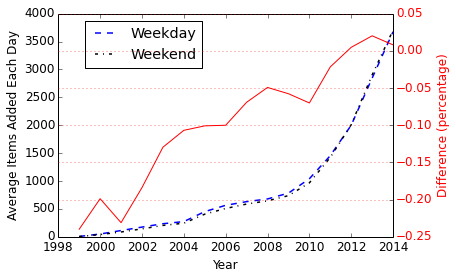
\includegraphics[width=0.45\textwidth]{weekday.png}
\end{figure}

\subsubsection{Normal days and Holidays}

In this section we measure how the items are added in the wish lists during holidays and normal days. As there are many unofficial or regional holidays, our study considers only nation-wide federal holidays. There are totally 10 qualified holidays. These holidays (http://www.usa.gov/citizens/holidays.shtml) and the date of the holidays are listed in Table~\ref{tb:holiday}.

\begin{table}[!ht]
\centering
\caption{U.S Federal Holidays}
\label{tb:holiday}
\begin{adjustbox}{max width=.45\textwidth}
\begin{tabular}{ll}
New Year's Day & January 1  \\
Birthday of Martin Luther King, Jr. & third Monday in January  \\
Washington's Birthday & third Monday of February  \\
Memorial Day & last Monday of May \\
Independence Day & July 4  \\
Labor Day & first Monday of September  \\
Columbus Day & second Monday in October  \\
Veterans Day & November 11  \\
Thanksgiving Day & fourth Thursday in November  \\
Christmas Day & December 25  \\
\end{tabular}
\end{adjustbox}
\end{table}

We analyze the data in 2 dimensions. First, We measure the items added in these holidays and compare the average items added in holidays and normal days. Then we compare the added items among different holidays. When calculating items added in a certain holiday, we consider the nearest consecutive 5 days. That is to say, we include the previous 2 days and the next 2 days in our holiday shopping session. For example, the Christmas day is December 25. We will include December 23, December 24, December 25, December 26, December 27 in Christmas day calculation. As a result, calculate items added during a year in a little different manner -- we include the last 2 days in previous year because the 2 days are considered New Year's day. We do not include the first 2 days in the next year because there is no holidays in the end of Decembers.


\subsubsection{Holidays and Normal Days}
According to our data, people start to add items in their wish lists since 1999. We analyze the items added in normal days and holidays in each year by calculating the average items added in the 2 groups. Figure~\ref{year} shows the items added in normal days and holidays 


\begin{enumerate}
\item The items added in wish lists increase year by year, no matter in normal days or holidays. We believe that the reason behind is that electric commercial gains its popularity.
\item There is increase in number of items added during holidays. The average increase rate is 10.89\%. However, as the data for year 1999 is not sufficient to be representative, we exclude year 1999 in our calculation and eventually we conclude that there is around 5.9\% increase in holidays. 
\item Generally people do buy more stuff during holidays. However, the increase is very limited. In 2001, the items added during holidays are even less than normal days. 
\end{enumerate}


\begin{figure}[h!]
\centering
  \caption{Items Added in Normal Days and Holidays}{}
  \label{fig:holiday}
  \centering
    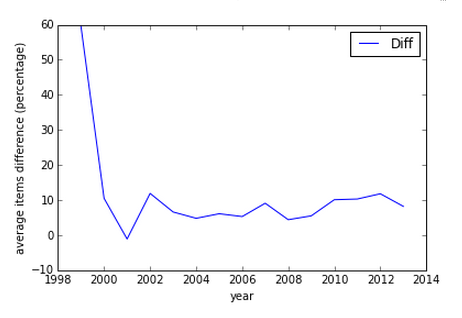
\includegraphics[width=0.45\textwidth]{holiday.png}
\end{figure}


\subsubsection{Different Holidays}
Previously we compared the shopping difference between holidays and normal days. We found that although people shop more in holidays, the increase is not that much. Our findings are against common impression that people do shop a lot in holidays, especially Thanksgiving and Christmas. We realized that it is rough to group all national holidays together to compare to normal days. We believe that holidays are also different from each other. For example people tend to shop more in Thanksgiving and Christmas. Therefore we compare different holidays in our study. Similarly, we include the last 2 days in the previous year in our analysis. There are 10 national holidays as introduced before. We again calculate the average number of items added in the nearest consecutive 5 days and compare to the average number of normal days. 

We use the data from year 1999 - 2014 and the year 2014 solely. We wish to show both the average case(from 1999-2013) and the current trend (only year 2013). We do not use data from Year 2014 because during the time of the study, the years 2014 has not been finished. Note that when computing the average item number added in normal days, we leave out all the holidays instead of simply leaving out the one that is being analyzed. The result is shown in Figure~\ref{alldiffholiday} for 1999-2013 and Figure~\ref{diffholiday} for the year 2013. In Figure~\ref{diffholiday}, The x-axis indicate the holidays accordingly (0-New Year's day, 1-Birthday of Martin Luther King, Jr, 2-Washington's Birthday, 3-Memorial Day, 4-Independence Day, 5-Labor Day, 6-Columbus day, 7-Veterans Day, 8-Thanksgiving day, 9-Christmas day).


\begin{figure}[!h]
\centering
\begin{minipage}{.25\textwidth}
  \centering
  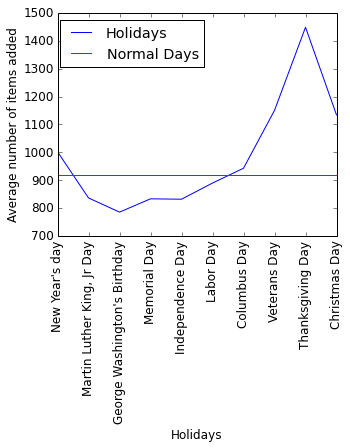
\includegraphics[width=.9\linewidth]{alldif.png}
  \captionof{figure}{Different Holidays in 1999-2014}
  \label{alldiffholiday}
\end{minipage}%
\begin{minipage}{.25\textwidth}
  \centering
  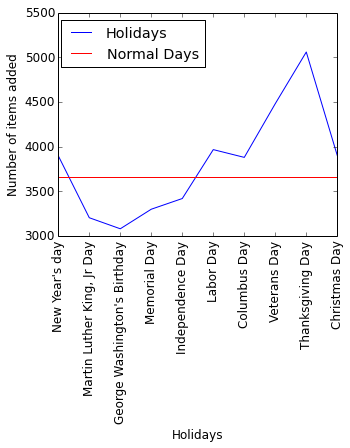
\includegraphics[width=.9\linewidth]{diff.png}
  \captionof{figure}{Different Holidays in 2014}
  \label{diffholiday}
\end{minipage}
\end{figure}


%\begin{figure}[H]
%%\minipage{0.5\textwidth}
%  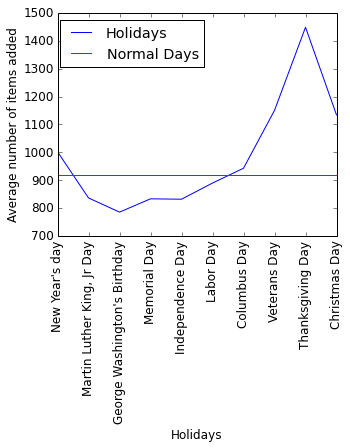
\includegraphics[width=\linewidth]{alldif.png}
%\caption{Different Holidays through 16 years}.
%\label{alldiffholiday}
%\endminipage\hfill
%\minipage{0.5\textwidth}%
%  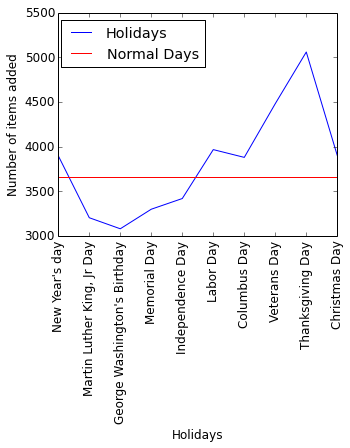
\includegraphics[width=\linewidth]{diff.png}
%\caption{Different Holidays in 2014}.
%\label{diffholiday}
%\endminipage
%\end{figure}


According to Figure~\ref{alldiffholiday} and Figure~\ref{diffholiday}, we find that holidays have huge difference between each other. In addition, we make the following observations:
\begin{enumerate}
\item The 2 figures match very well, which means that people do not tend to change their shopping behaviors at least during a short period of time. 
\item Some of the holidays are not much different from normal days (For example, Columbus Day). What is more, some of the holidays make the people less willing to add items in their wish lists. 
\item New Year's day, Veterans day, Thanksgiving, and Christmas day are 4 holidays that have quite obvious shopping increase. The result indicates that people tend to buy more stuff during the 4 holidays. The increase rate is 4.1\%, 25.2\%,72.8\%, and 30.2\% accordingly for all 15 years we analyzed. 
\item Among the 4 holidays, Thanksgiving day is the most shopping appealing holiday, which is 72.8\% higher than normal days. It is reasonable because people always get considerable discount during thanksgiving days. Christmas is the second most shopping appealing holiday because people always need to buy presents during Christmas.
\item At the first glance it is surprising that 4 holidays -- Birthday of Martin Luther King. Jr, Washington's Birthday, Memorial Day, Independence Day, and Labor day -- clearly have even less items added to user Wish Lists. The drop percentage is 10.7\%, 11.8\%, 9.0\%, 11.3\%, and 4.6\%. One possible reason is that People are more likely to be involved in other activities other than shopping during these holidays. 3 out of the 4 holidays are memorial days. Certainly these days are considered not good for shopping. 
\end{enumerate}

We believe our quantitative results are helpful in guiding merchant marketing strategies and targeted advertising. 

\section{Privacy Information Identification}

From our measurement study, we have studies 3 dimensions of user shopping preference -- 1)What to buy 2)When to buy 3)Price.

From our study of shopping preference difference, it has been clear that different people have different shopping preference. One question is: Can we identify user personal information from the their Wish Lists. That is to say, Items added in Wish Lists have potential to leak personal information. We explore the possibility using machine learning to help identify user personal information from their Wish Lists.
\subsection{Information in list-description}
To successfully identify the user personal information. One challenge we face is how to obtain the ground truth of the user. There are several possible ways to find out the result. First, Services such as yahoo people search can be used as ground truth at a reasonable monetary cost. We can input the name and location information in the search engine to identify a user. Second, similar to the first approach, we can search people in online social networks such as Facebook or Twitter. Third, we can use the user list-description as the ground truth. Users sometimes expose personal information in their list-description and we can take advantage of it.

The first approach does not really provide an accurate result since the information given is not rigorous enough to identify the exact person. If wrongly identified, it has much negative impact on the identification process, which is by itself not very accurate already. The second approach is similar to the first one. It is even more inaccurate. Due to the unreliable nature of the first 2 approaches, we took the third approach. Besides the accuracy, collecting ground truth from list-descriptions have the benefit of not depending on external data source. Recall that we collect items for only users with list-descriptions. All our 20,099 users collected have list-descriptions. Note that there are also limitations for the third approach. For example, the list-description is plain-text, making it hard to process and analyze. Secondly, there may not always be useful information in list-descriptions.

We assume that everybody is telling the truth in the list-descriptions. If somebody is lying, we do not have a way to identify it. However, it is meaningless for a user to lie in list-descriptions since lying there will not bring them any benefit. If a user concerns his/her privacy, he/she can simply leave the list-description blank instead of lying.

Among the users who have list-descriptions, 233,595 words are found (44,387 punctuations are excluded). The average number of words in list-descriptions is 11.6. We can see that the list-descriptions are not long -- basically the length of a normal sentence. While there are scattered long list-description (the longest list-description has 682 words), more than half of the list-descriptions have length less than or equal to 6 (10,592 out of 20,099). And only 29.9\% of the list-descriptions have over 10 words. Considering that there are even less words that carry information, One possible consequence is that there might not be enough information in one list-description to identify personal information.

Next we retrieve information from list-descriptions. 

One way to retrieve information is to search the keyword. If a keyword appears in one user's self-description, there is high probability that the user is related to the keyword. For example, if a keyword "college" appears in the self-description, the user is likely to have a college degree. 

We used Stanford Part-of-Speech (POS) tagger \cite{toutanova2003feature} to tag the user list-descriptions to retrieve useful information. There are a number of tags a word can belong to. However, we only focus on noun-family words (with tag NN, NNS, NNP, and NNPS in Stanford POS tagger). The reason behind is that most of the nouns carry certain amount of information while most of other words do not carry useful information. 

There are totally 95,359 out of all 233,595 words (around 40.8\%) belonging to the noun family. The ratio of nouns is quite large. The most frequent ones are listed in Table~\ref{tb:freq}

\begin{table}[!ht]
\centering
\caption{Frequent Nouns IN list-descriptions}
\label{tb:freq}
\begin{tabular}{lll}
 Rank & Item Type & frequency\\
 1 & s & 1498   \\
 2 & love & 1327   \\
 3 & m & 1314   \\
 4 & university & 1098   \\
 5 & music & 1095   \\
 6 & list & 1064   \\
 7 & books & 1001   \\
 8 & school & 659   \\
 9 & movies & 652   \\
 10 & t & 628  \\
 11 & games & 593  \\
 12 & things & 553   \\
 13 & college & 495  \\
 14 & stuff & 443  \\
 15 & work & 419   \\
 16 & fan & 411  \\
 17 & wish & 389  \\
 18 & video & 380  \\
 19 & history & 371  \\
 20 & photography & 353  \\
\end{tabular}
\end{table}

From Table~\ref{tb:freq} We can see that except for meaningless single characters ("s" and "m" in this case), the noun family words carry some information of a user. The information involves hobbies (such as music, books, movies, etc) and education level (such as university, college). These words can be used as keywords in the information retrieval step. On the other hand, if we look into the verbs, we will find the most popular 20 verbs are "is",  "am",  "have",  "are",  "live",  "be",  "love",  "buy",  "want",  "enjoy",  "know",  "used",  "do",  "don",  "get",  "married",  "go",  "went",  "read",  "loves",  and "was". Except "married", the other words can not assist us to find any useful information about a user.
\subsection{Information Identification}
We do personal information identification on a subset of users who have more than 30 items in their wish lists in our dataset. We filter part of the users out because they do not have sufficient information in their Wish Lists. After the filtering, we have 13,464 users as our target users. We choose users with certain keywords in their list-descriptions in the user pool. We use the portion of different types of products,  in user wish lists as input to the classifier. Therefore we have an input vector of length of 50. We use SVM classifier to train and test the data. 80\% of our data is used as training data and the rest of 20\% of the data as testing data. The personal information identification process is binary, which means that we use only 2 classes in each identification cycle. The reasons for having only 2 classes. It is reasonable to have 2 classes in a classifier. We intend to answer questions like "Is he a professor?", "Does he have a university diploma" or "Does he like hiking?". A prediction of the answer is very helpful in identifying a user. We try 2 different types of personal information -- 1) gender 2)hobbies

\subsection{gender}
There are only 2 genders in general, it is natural to have only 2 classes. To save the training resource while maintaining high representation, we chose 389 males and 168 females as our dataset. We used the first 80\% person as the training set and the rest as the test set. The ground truth comes from the name of the users. We identify a user "male" if this user is using a male name in the profile. females are identified using a similar approach. As a result, the success rate to classify whether a given user is a male or female is around 84\%.
We can see that the classifier works pretty well in the case of gender, which means that given only the Wish List information of a user, we can identify whether this user is male or female with pretty high certainty.

\subsection{Hobbies}
Afterwards, We use hobbies as examples, we choose all pairs of hobbies in the top 20 nouns. 7 keywords are selected. They are -"music", "books", "movies", "games", "video", "history", and "photography" and try to differentiate users between any pair of them. The success rate between any pair of them is shown in Table~\ref{tb:hobby}

\begin{table}[!ht]
\centering
\caption{Success Rate of Hobbies}
\label{tb:hobby}
\begin{adjustbox}{max width=.5\textwidth}
\begin{tabular}{llllllll}
            & music & books & movies & games & video & history & photography \\
music       & NA    & 0.506 & 0.653  & 0.713 & 0.691 & 0.772   & 0.743       \\
books       & 0.506 & NA    & 0.631  & 0.667 & 0.647 & 0.526   & 0.807       \\
movies      & 0.653 & 0.631 & NA     & 0.617 & 0.617 & 0.762   & 0.662       \\
games       & 0.713 & 0.667 & 0.617  & NA    & 0.521 & 0.776   & 0.703       \\
video       & 0.691 & 0.647 & 0.617  & 0.521 & NA    & 0.777   & 0.700       \\
history     & 0.772 & 0.526 & 0.762  & 0.776 & 0.777 & NA      & 0.680       \\
photography & 0.743 & 0.807 & 0.662  & 0.703 & 0.700 & 0.680   & NA         
\end{tabular}
\end{adjustbox}
\end{table}

We can see that the success rate can be high (80.7\%) or even no better than guessing (50.6\%). Such big variance may be due to the relativity of different hobbies. When 2 hobbies are not much related, we can find the success rate be usually higher than 70\%. For example, "history" has very limited relativity to other hobbies except for "books". We can see from the table that history has higher success rate except for the "books" entry because history relates to books pretty much. It is difficult to have further increase in success rate because people often have more than 1 hobbies. Therefore one person may belong to both group, which will have quite negative impact on the result.

We conclude that wish lists are helpful to identify a user's hobby. However, depending solely on wish lists are not a very reliable option to identify user hobbies. 
\section{Discussion}
\subsection{Data Limitation}
There is certain limitation in the data of this study. One problem is that the data may be biased. User wishlists are not always public -- users have the ability to change the accessibility of their wish lists (although the default is public). Therefore privacy-aware users may choose to publicize some of their wish lists while keep other wish lists from strangers. Besides, users may choose not to share certain items in their wish lists. For example, privacy-sensitive items such as pregnancy test, firearm-related products, and medicine \& drugs. In our work we can only retrieve the product in public wish lists. The data may not be 100\% representative of one users' shopping behavior.

\subsection{Personal Information Identification}
We have done a pilot study on predicting user gender from their wishlists. We now discuss the potential to use wishlists to identify other types of personal information. To conduct such experiments, first we may need to identify the ground truth. Other than the several available information, we can extract useful information in the list-descriptions. However, it involves accurate human language processing and may require much more effort. Some other way to obtain ground truth is to search online social network, which is shown to be fairly easy~\cite{krishnamurthy2009leakage}. In order to maintain high accuracy, finer-granularity wishlist information may be retrieved. For example, subcategories, ranking of items, timing factor could be effective features to create better machine learning models. We believe identifying more personal information using wishlists is very promising, which will be left as a future work. 


\section{Related Work}

There are a large amount of works that have been done to learn plain text. \cite{de2001mining} mines e-mail content for author identification. They study an extended set of email document features, which include structure, linguistic patterns, etc. They use SVM learning algorithm to differentiate the authors of emails. \cite{pang2002thumbs}presented algorithm for mining users' opinions of an item from their reviews of the items, classifying documents in overall sentiment. They use keywords appearing in the user comments of an item to infer whether the user like this item or not and to what extend do they like/dislike the item.

\cite{Lee:2010:USS:1835449.1835522} does statistical analysis of the properties of spam profiles collected from social network communities for creating spam classifiers to actively filter out existing and new spammers. \cite{dave2003mining} describes the system infrastructure, identify the unique properties of list of product attributes and develops a method for automatically distinguishing between positive and negative reviews in Movie Lens to link forum posts to mentioned items. \cite{kraft2007mashing}attempts to do on a set of Amazon wish lists spiders from web. They started by doing a wish lists search of people names(first names and nicknames from the baby names databases) and then retrieve the results linking to the wish lists of the first 25 matches. 

\section{Conclusion}
In this paper, we investigate Amazon wishlists, where users store their desired products. We collect over 30,000 users' complete wishlsits and took a 2-step approach to analyze our data. First we try to measure the user behavior from their wish lists by analyzing wishlists in multiple dimensions. Our result shows that there is huge discrepancy between male and female online shopping pattern. The 2 groups differ in both preferred product categories and prices. Furthermore, we investigate user shopping preference taking time as a factor. We reveal that users are in fact not shopping significantly more during holidays or weekends in terms of online shopping. We also investigate different holidays that are shopping appealing or repelling. We highlight that although there are certain holidays are very shopping involving, over half of the national holidays have no increment or even lower shopping favor than normal days. After studying user shopping pattern, we try to identify personal information from list-descriptions or items in the lists. We apply simple human language processing on the plaintext in list-descriptions to generalize the information users tend to expose. Beside the information users mentioned themselves, we also explore the possibility to infer user personal information based on their wishlists. To this end, we selected representative features from wishlists and use SVM to infer user gender. Our results show that given a user that has abundant wishlists, we can predict the user's gender with fairly high accuracy.



\IEEEpeerreviewmaketitle

\bibliographystyle{abbrv}
\bibliography{ref}


\end{document}


